%\begin{figure*}[t]
%		\begin{minipage}{0.32\linewidth}
%			\centering
%			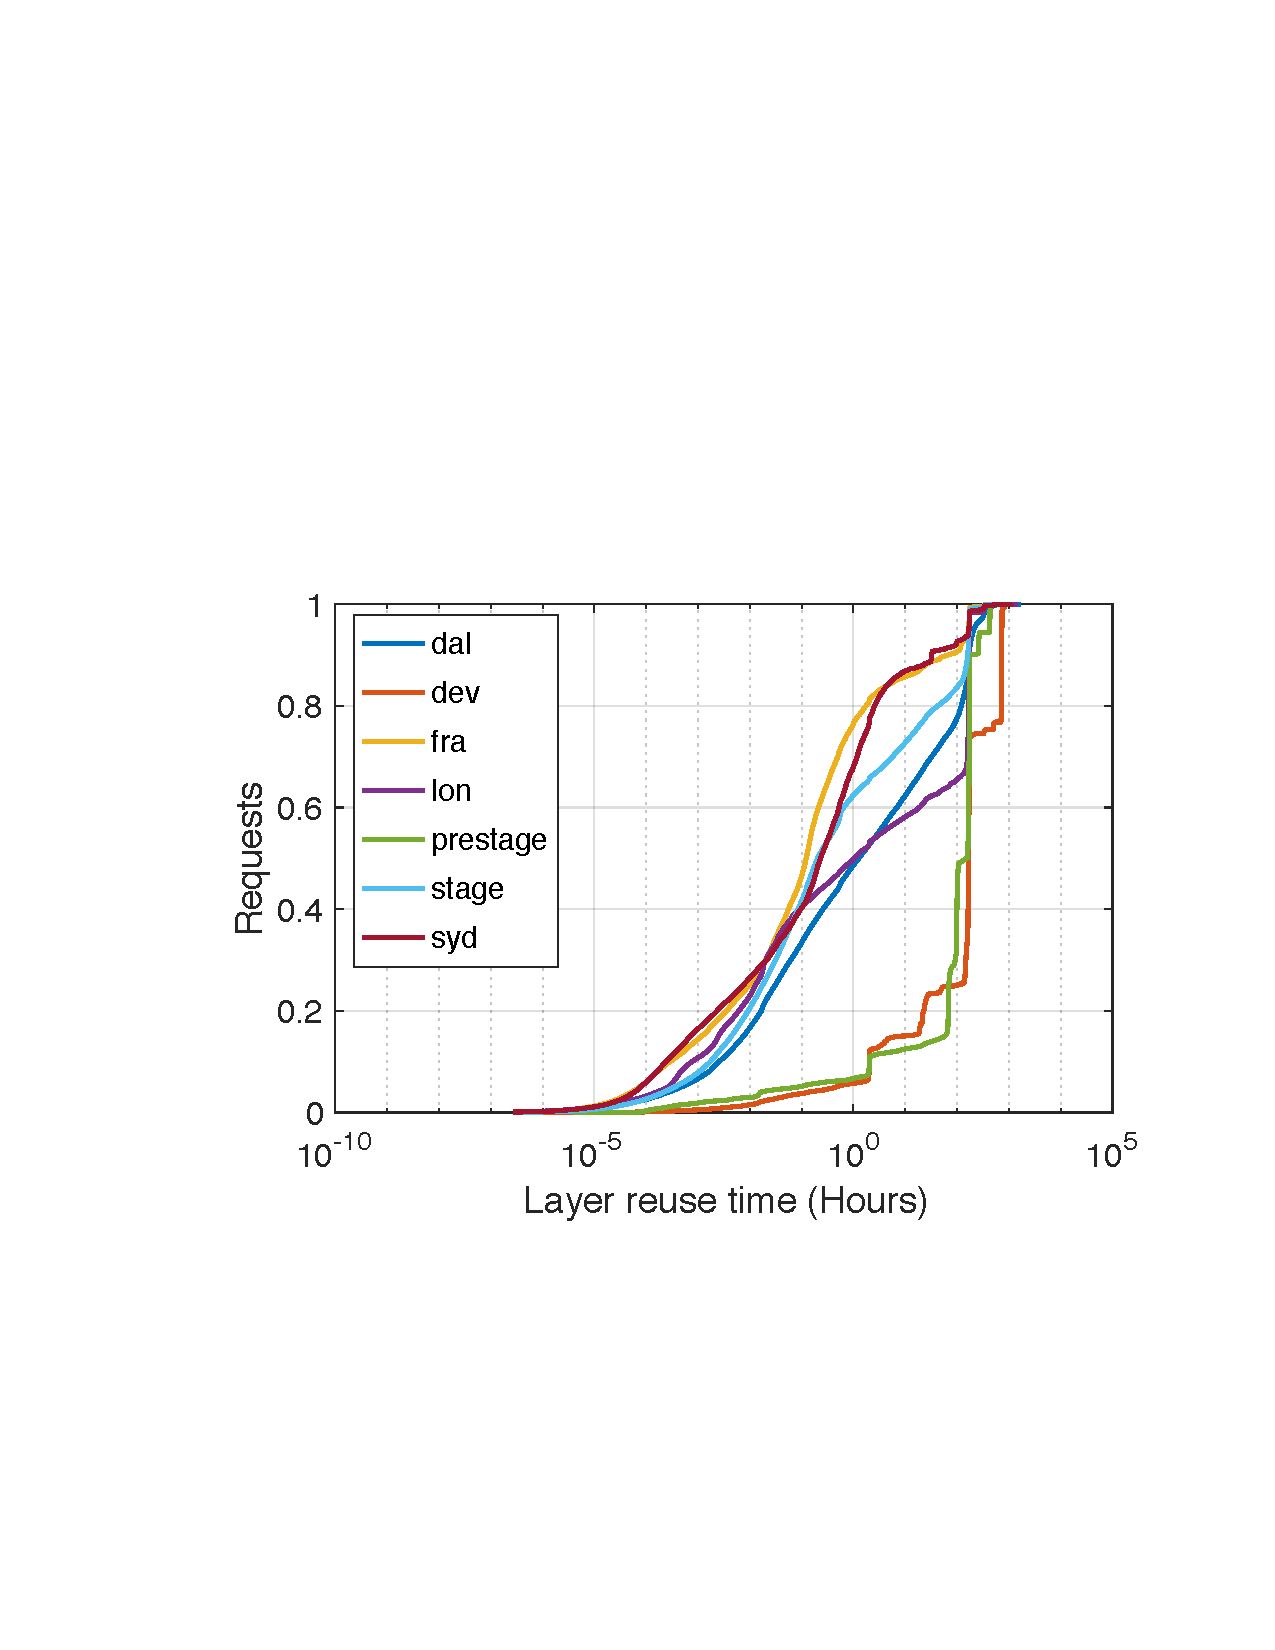
\includegraphics[width=1\textwidth]{graphs/layer-reusetime.pdf}
%		%	\caption{CDF of layer reuse time.}
%		%	\vspace{-3pt}
%			\label{fig:layer-reuse}
%		\end{minipage}
%			\begin{minipage}{0.32\linewidth}
%				\centering
%				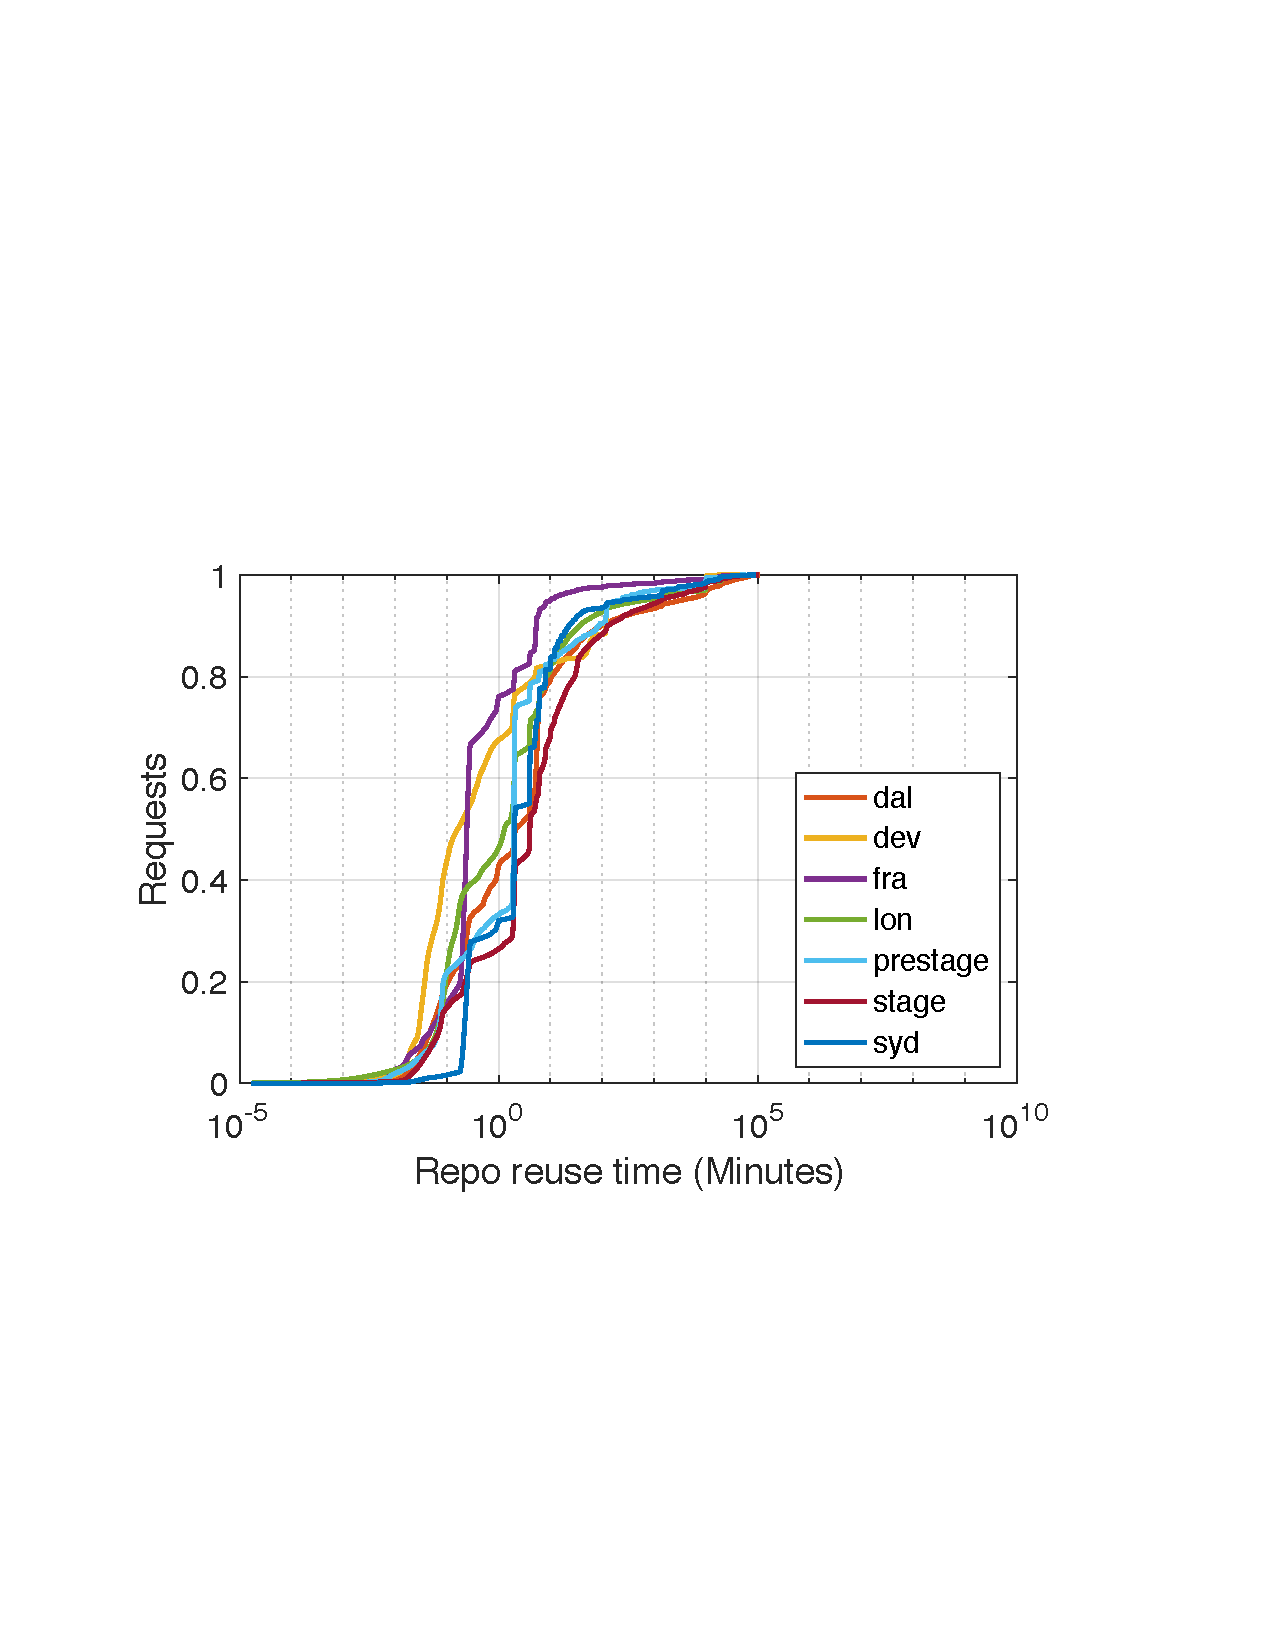
\includegraphics[width=1\textwidth]{graphs/repo-reusetime.pdf}
%			%	\caption{PDF of repository reuse time.}
%				%	\vspace{-3pt}
%				\label{fig:repo-reuse}
%			\end{minipage}
%		\begin{minipage}{0.32\linewidth}
%			\centering
%			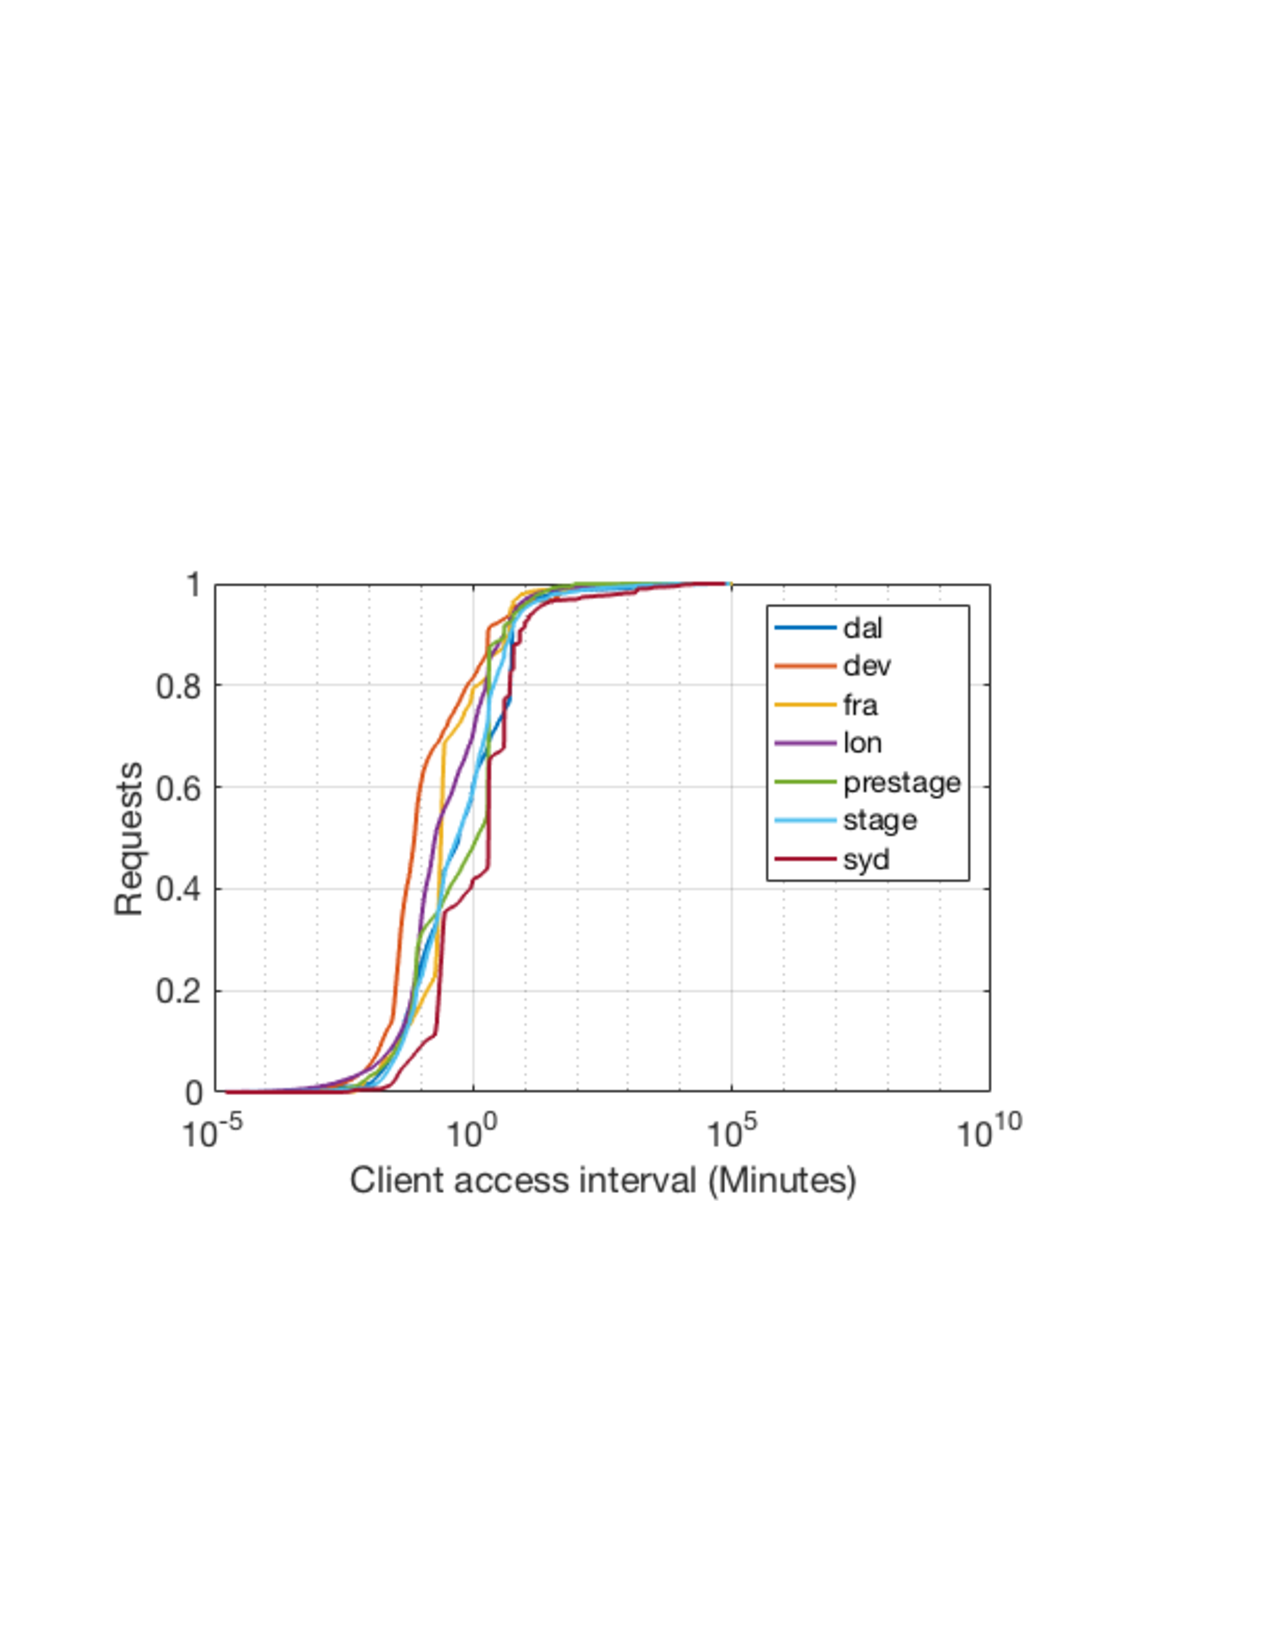
\includegraphics[width=1\textwidth]{graphs/user-intervals.pdf}
%			%\caption{PDF of client access intervals.}
%			%	\vspace{-3pt}
%			\label{fig:user-interval}
%		\end{minipage}
%	\caption{CDF of reusetime for layers, repositories and clients' access intervals.}
%	\label{fig:layer-reuse}
%\end{figure*}

%\begin{figure}[t]
%	\centering
%	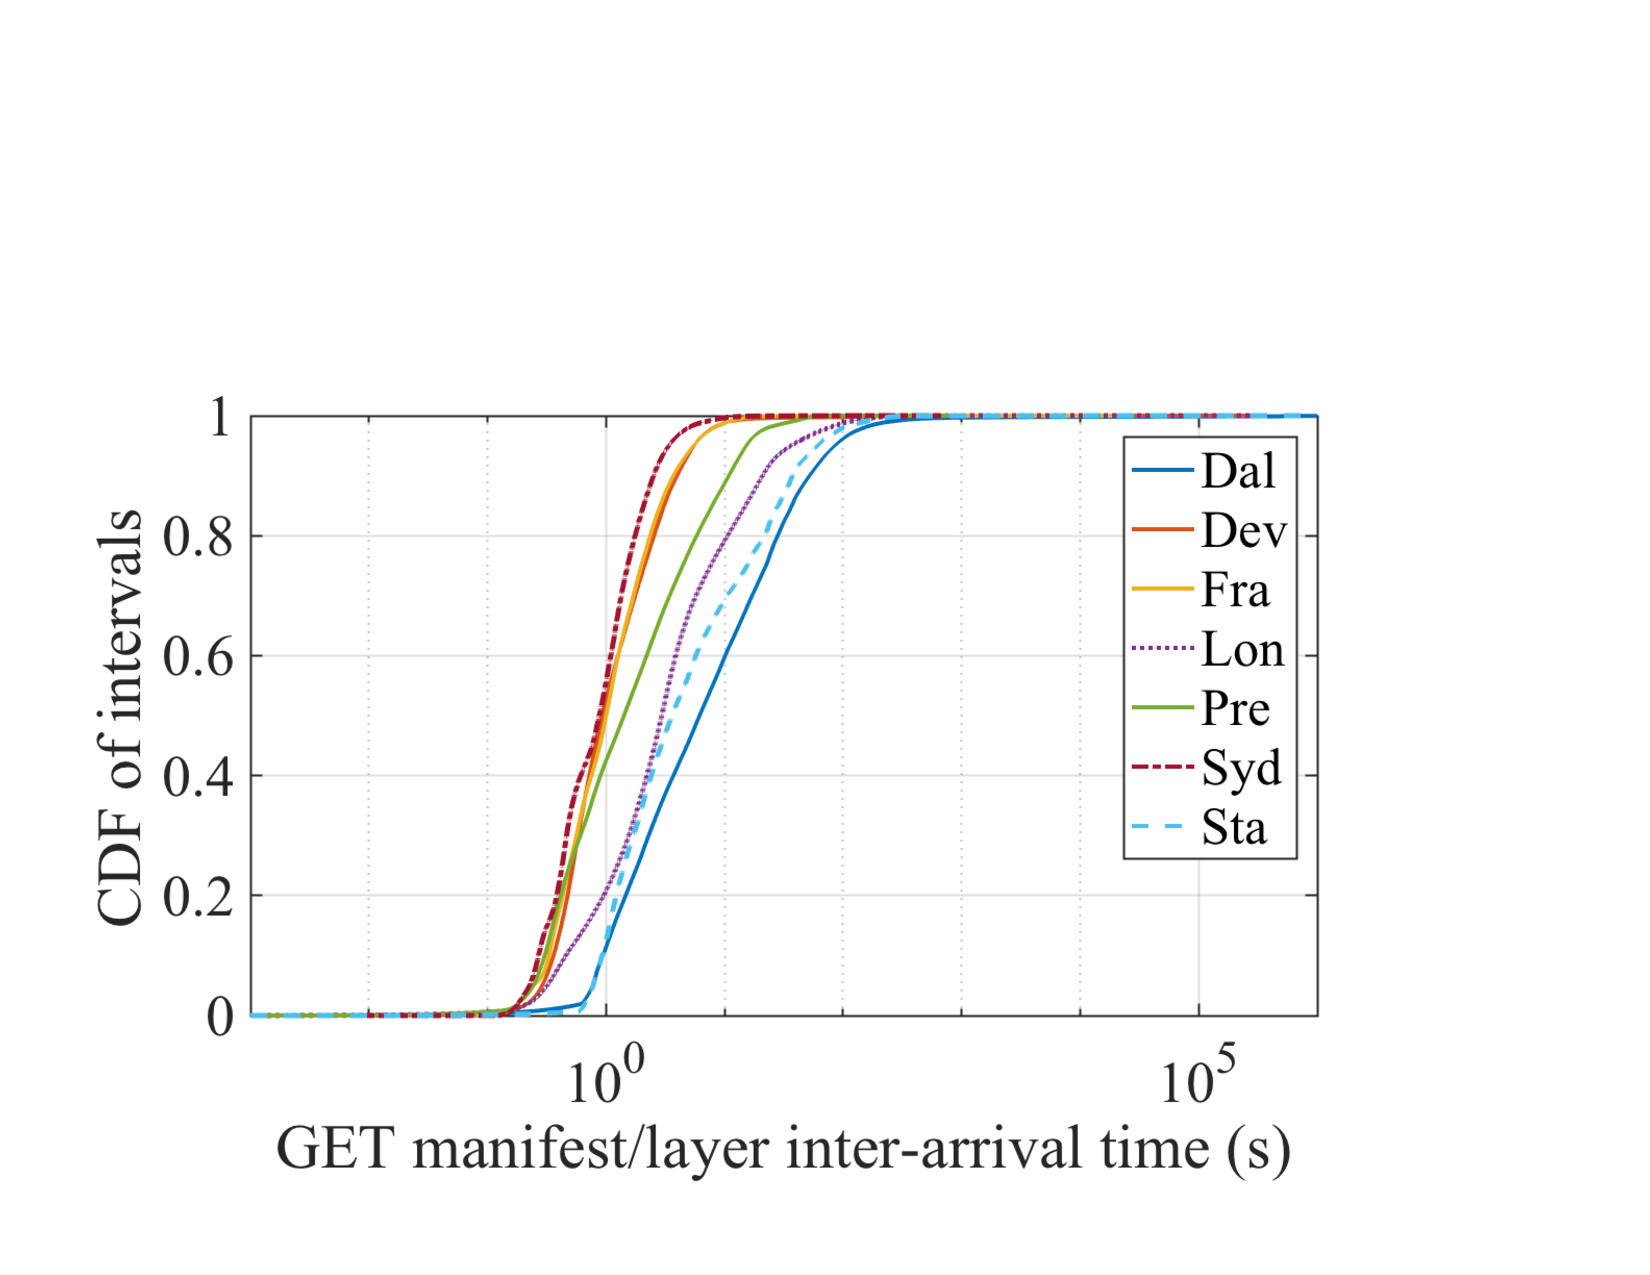
\includegraphics[width=0.3\textwidth]{graphs/GML-intervals.pdf}
%	\caption{Intervals between \texttt{GET} manifest request and \texttt{GET} layer request}
%	%	\vspace{-3pt}
%	\label{fig:intervals}
%	
%\end{figure}

%\begin{figure*}[!t]
%	\centering
%	\subfigure[Layer repull count]{
%		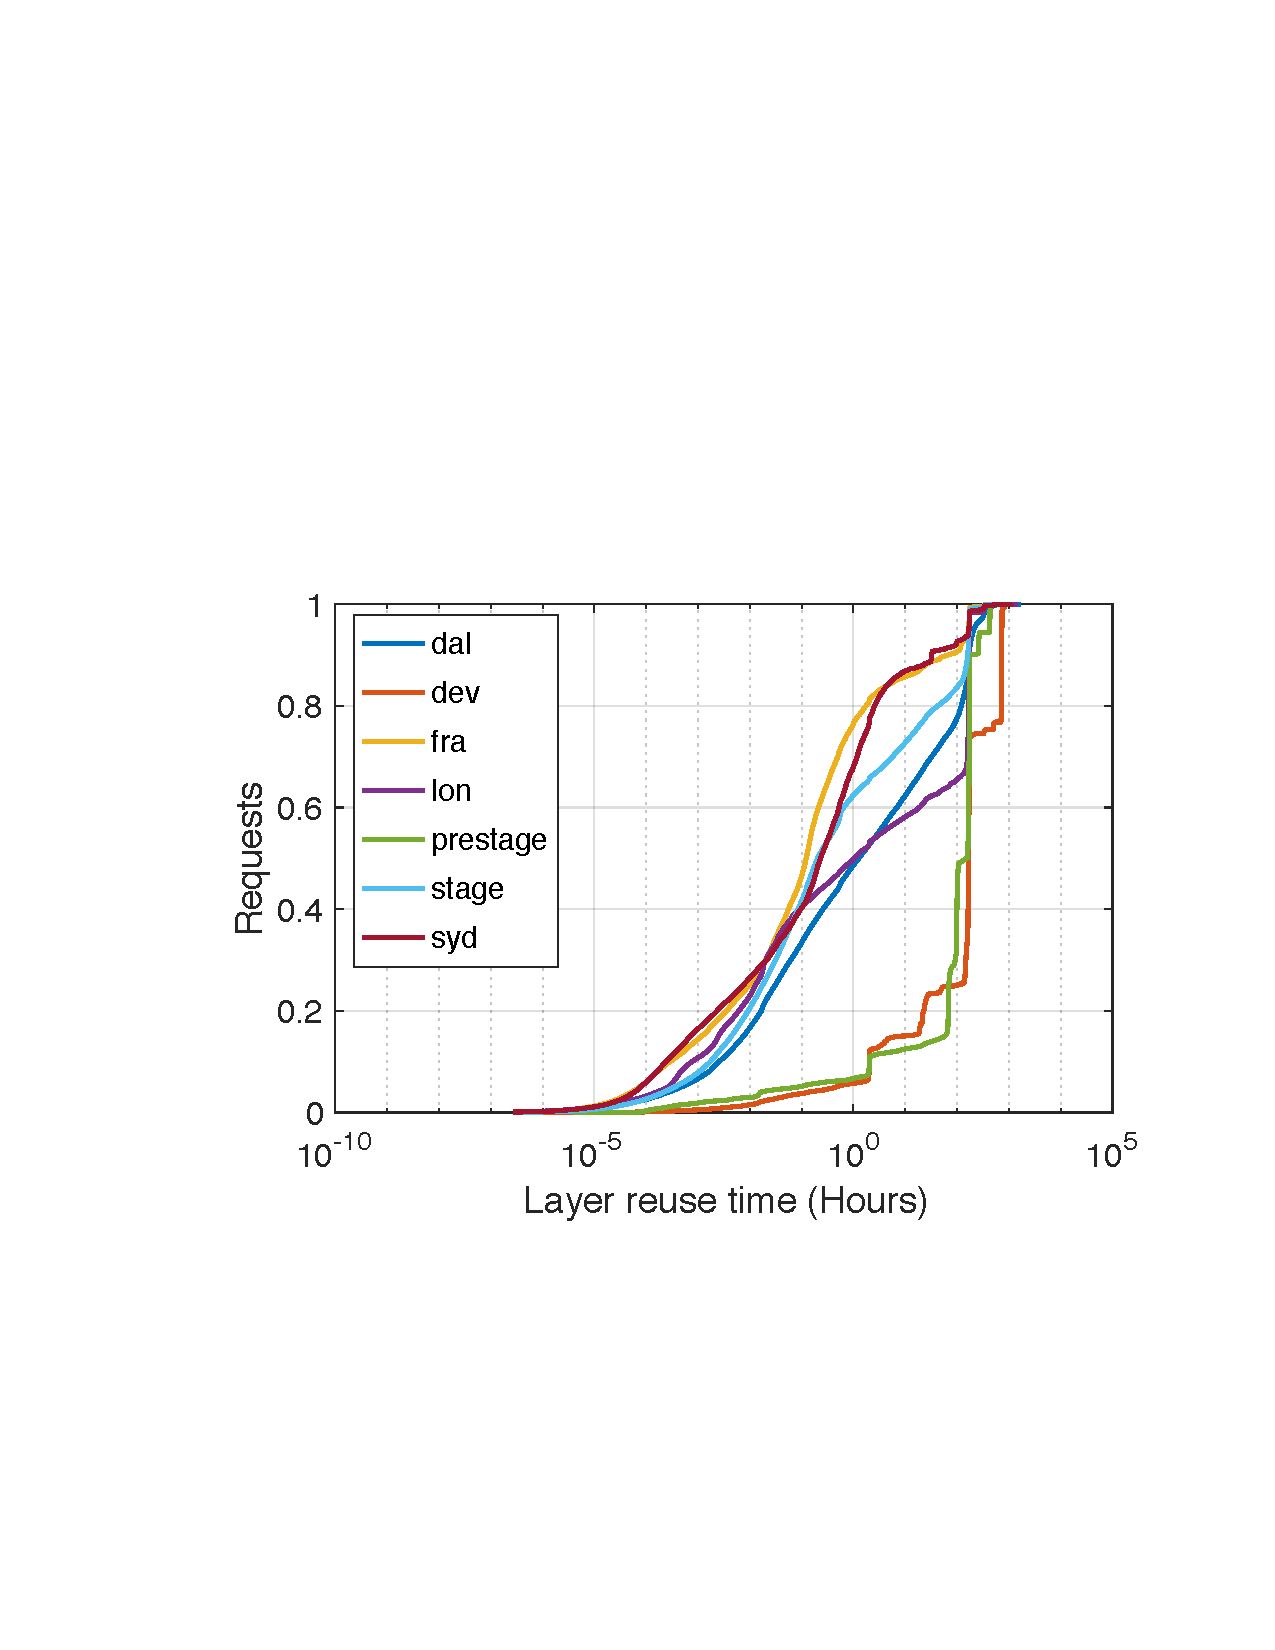
\includegraphics[width=0.2\linewidth]{graphs/layer-reusetime.pdf}
%			\label{fig:layer-reuse}
%	}
%	\subfigure[Repository repulling probability]{
%		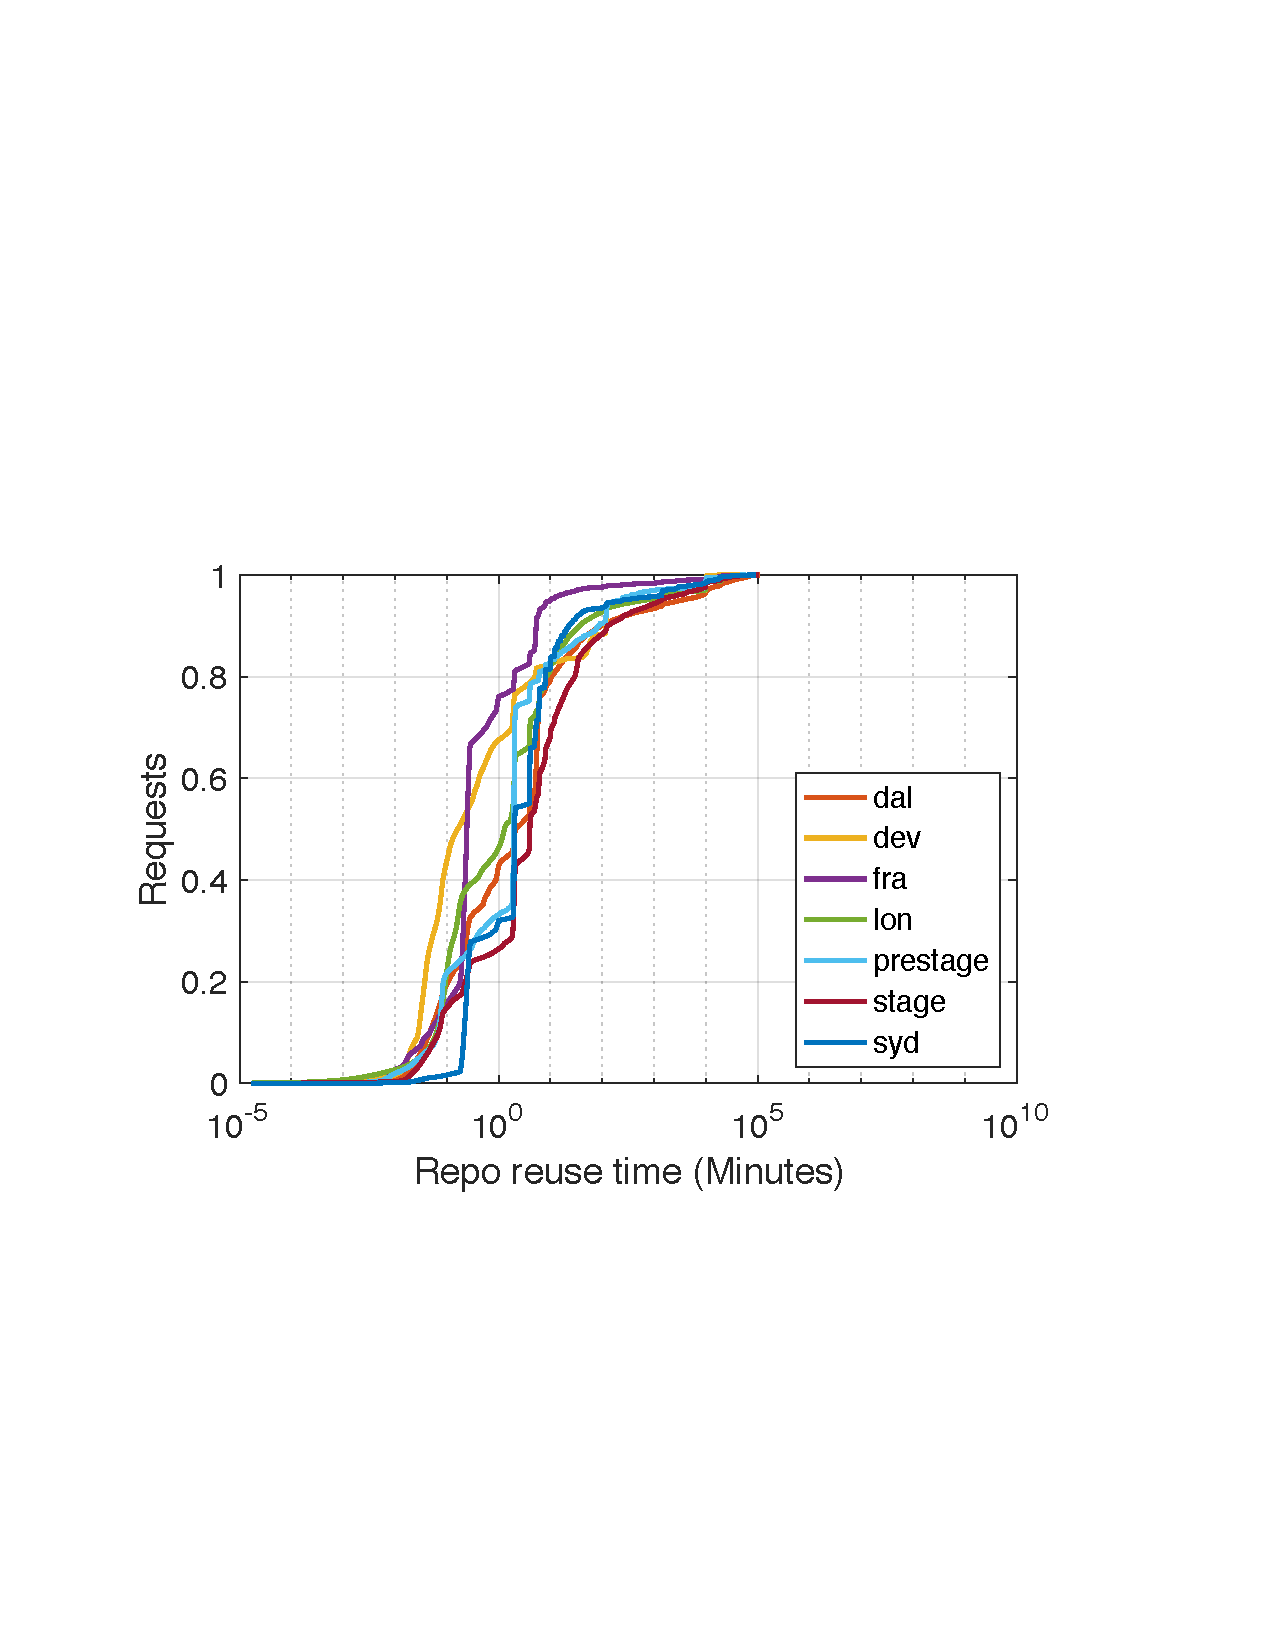
\includegraphics[width=0.2\linewidth]{graphs/repo-reusetime.pdf}
%				\label{fig:repo-reuse}
%	}
%	\subfigure[Client repulling probability]{
%		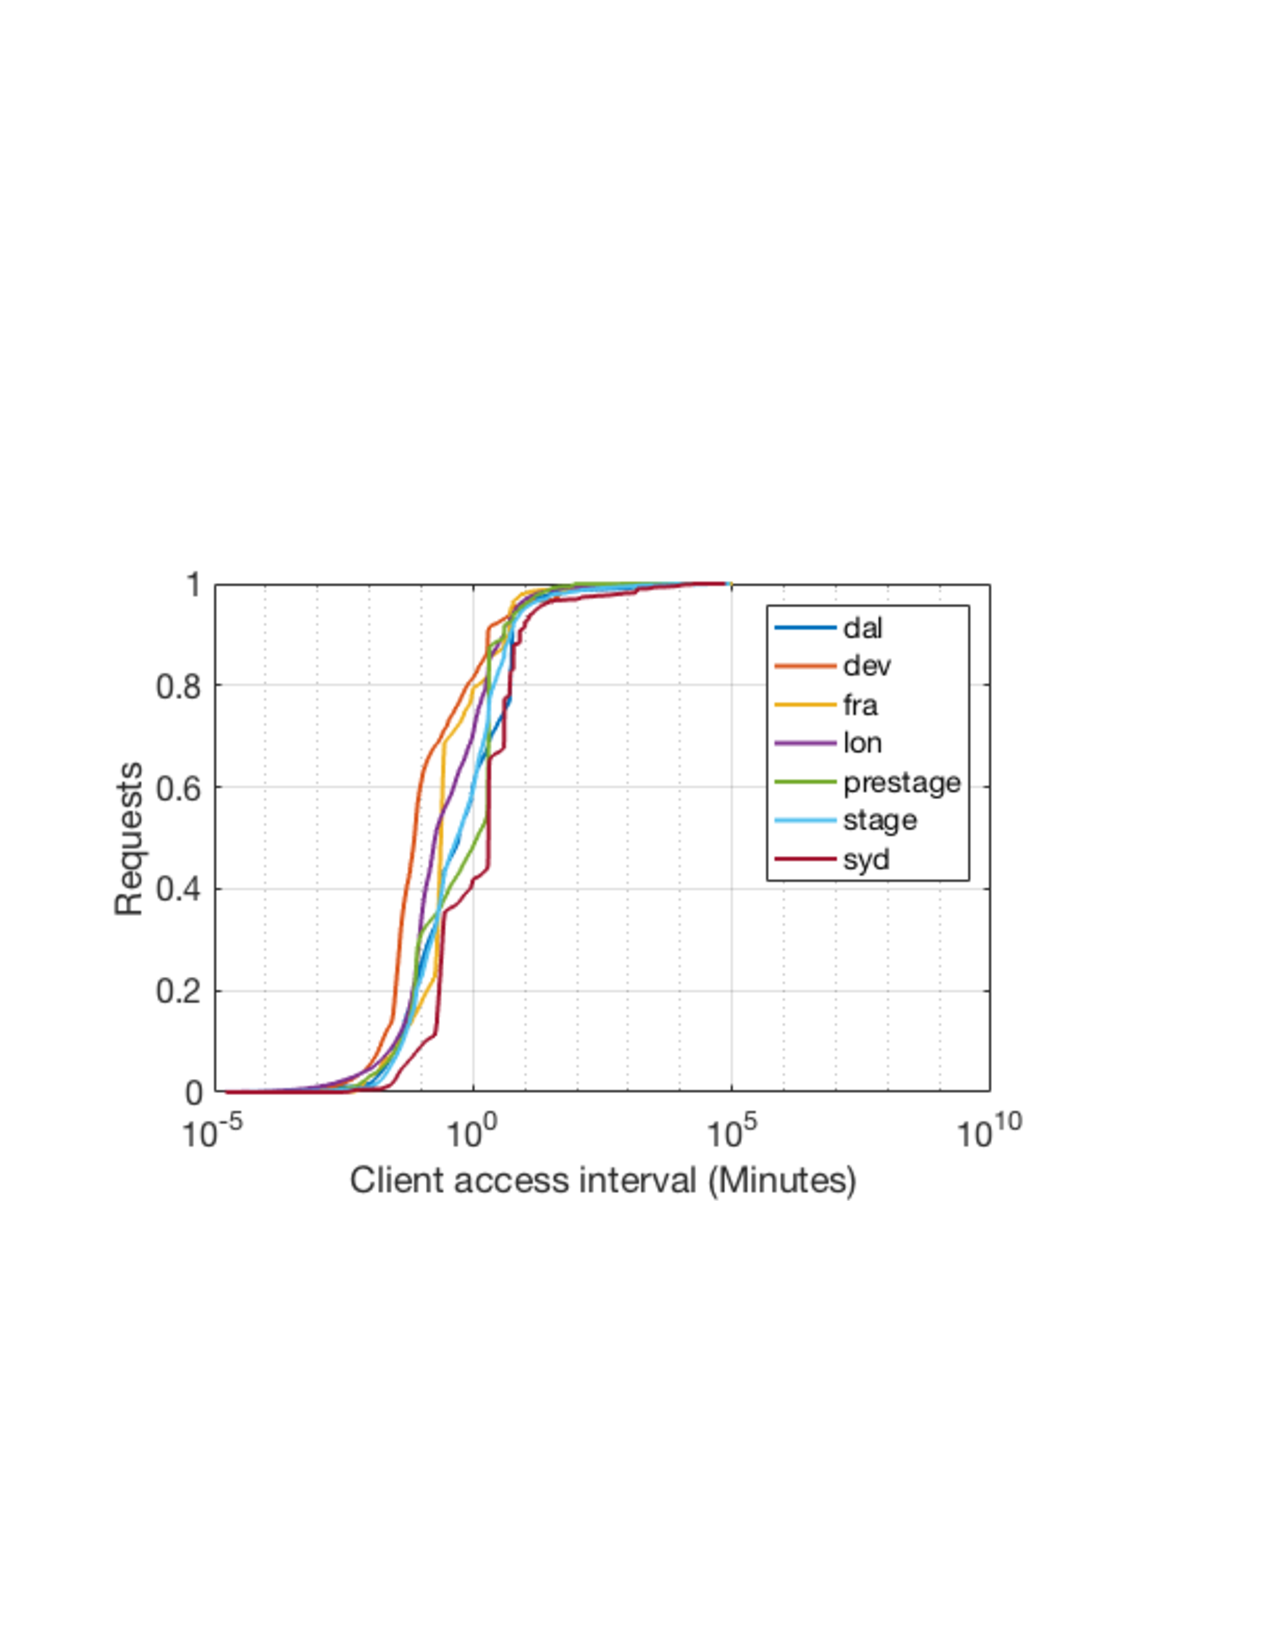
\includegraphics[width=0.2\linewidth]{graphs/user-intervals.pdf}
%			\label{fig:user-interval}
%	}
%	\caption{CDF of reusetime for layers, repositories and clients' access intervals.}
%	\label{fig:fig-reuse}
%\end{figure*}

%\begin{figure}[t]
%	\centering
%	\begin{minipage}{0.26\textwidth}
%		\centering
%		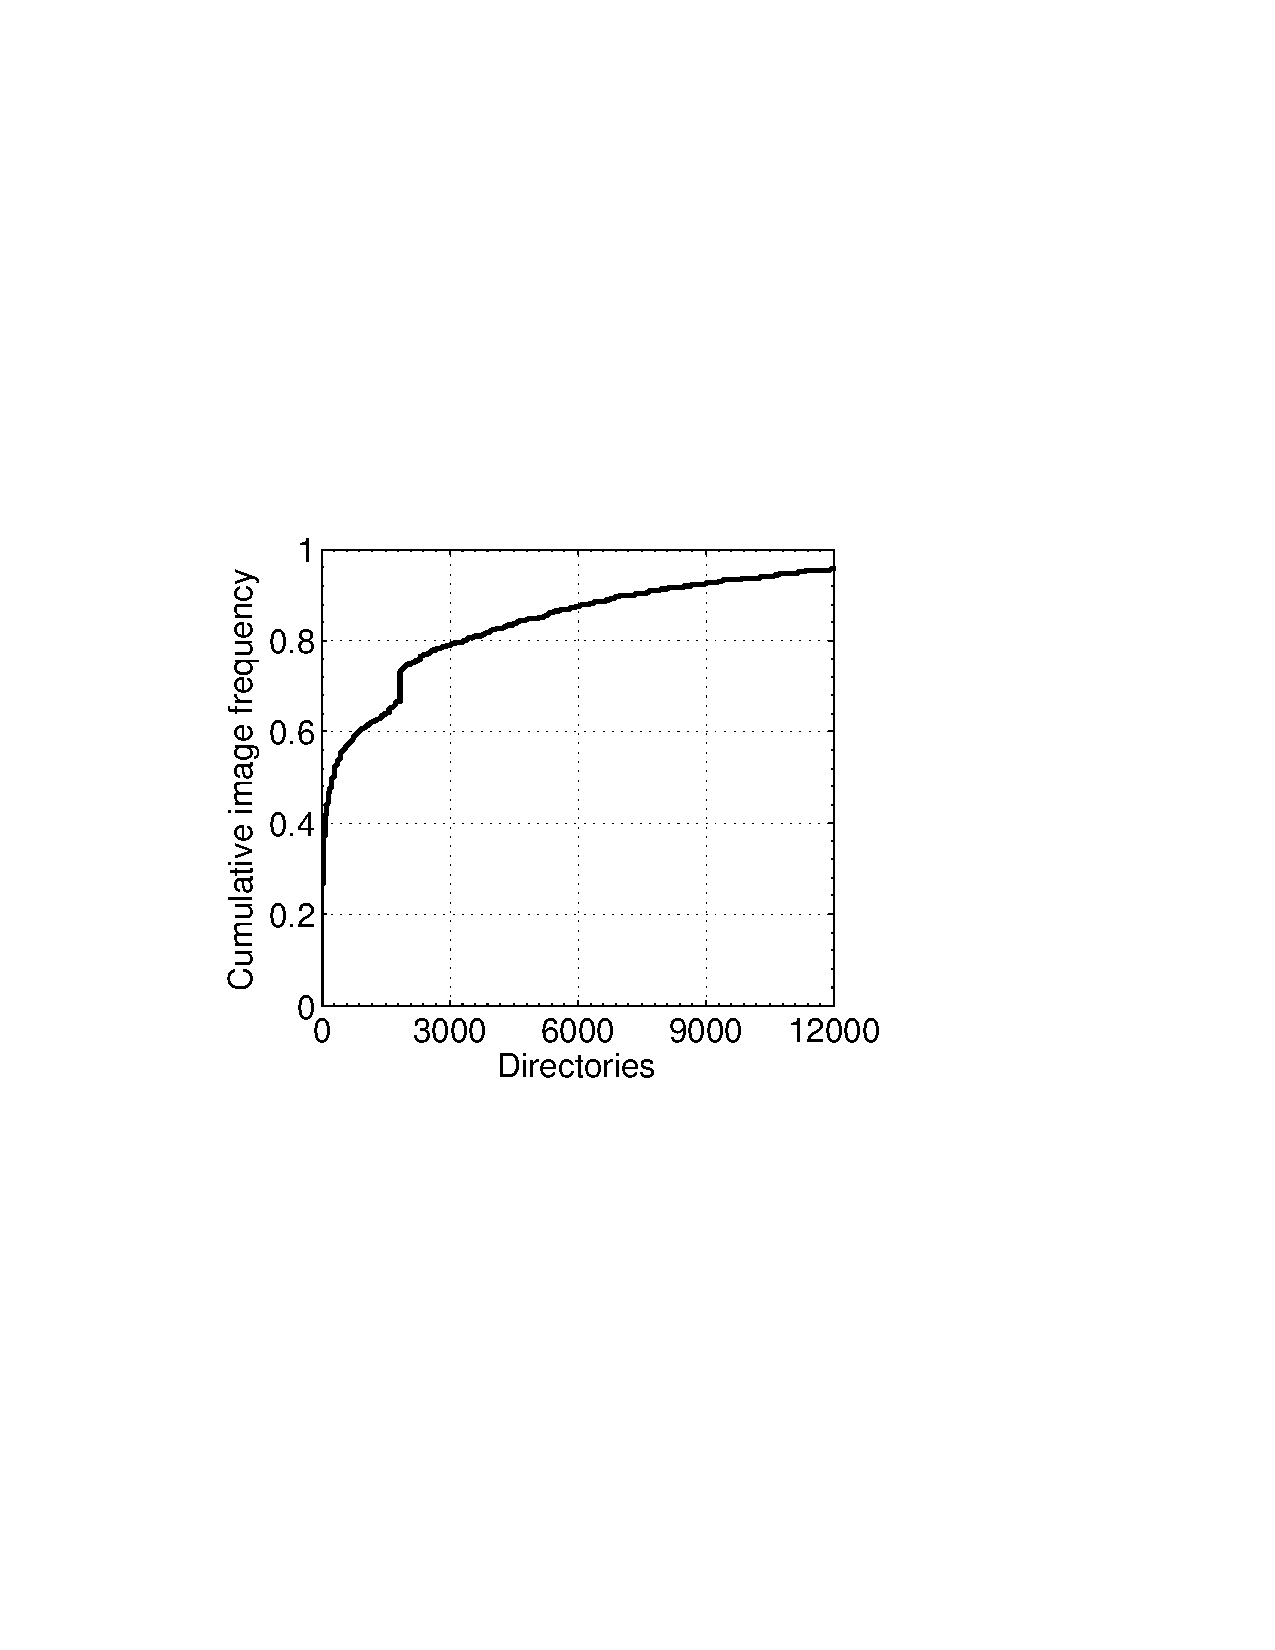
\includegraphics[width=1\textwidth]{graphs/dir.pdf}
%		\caption{CDF of images by\newline directories}
%		\label{fig-dir}
%	\end{minipage}%
%	\begin{minipage}{0.24\textwidth}
%		\centering
%		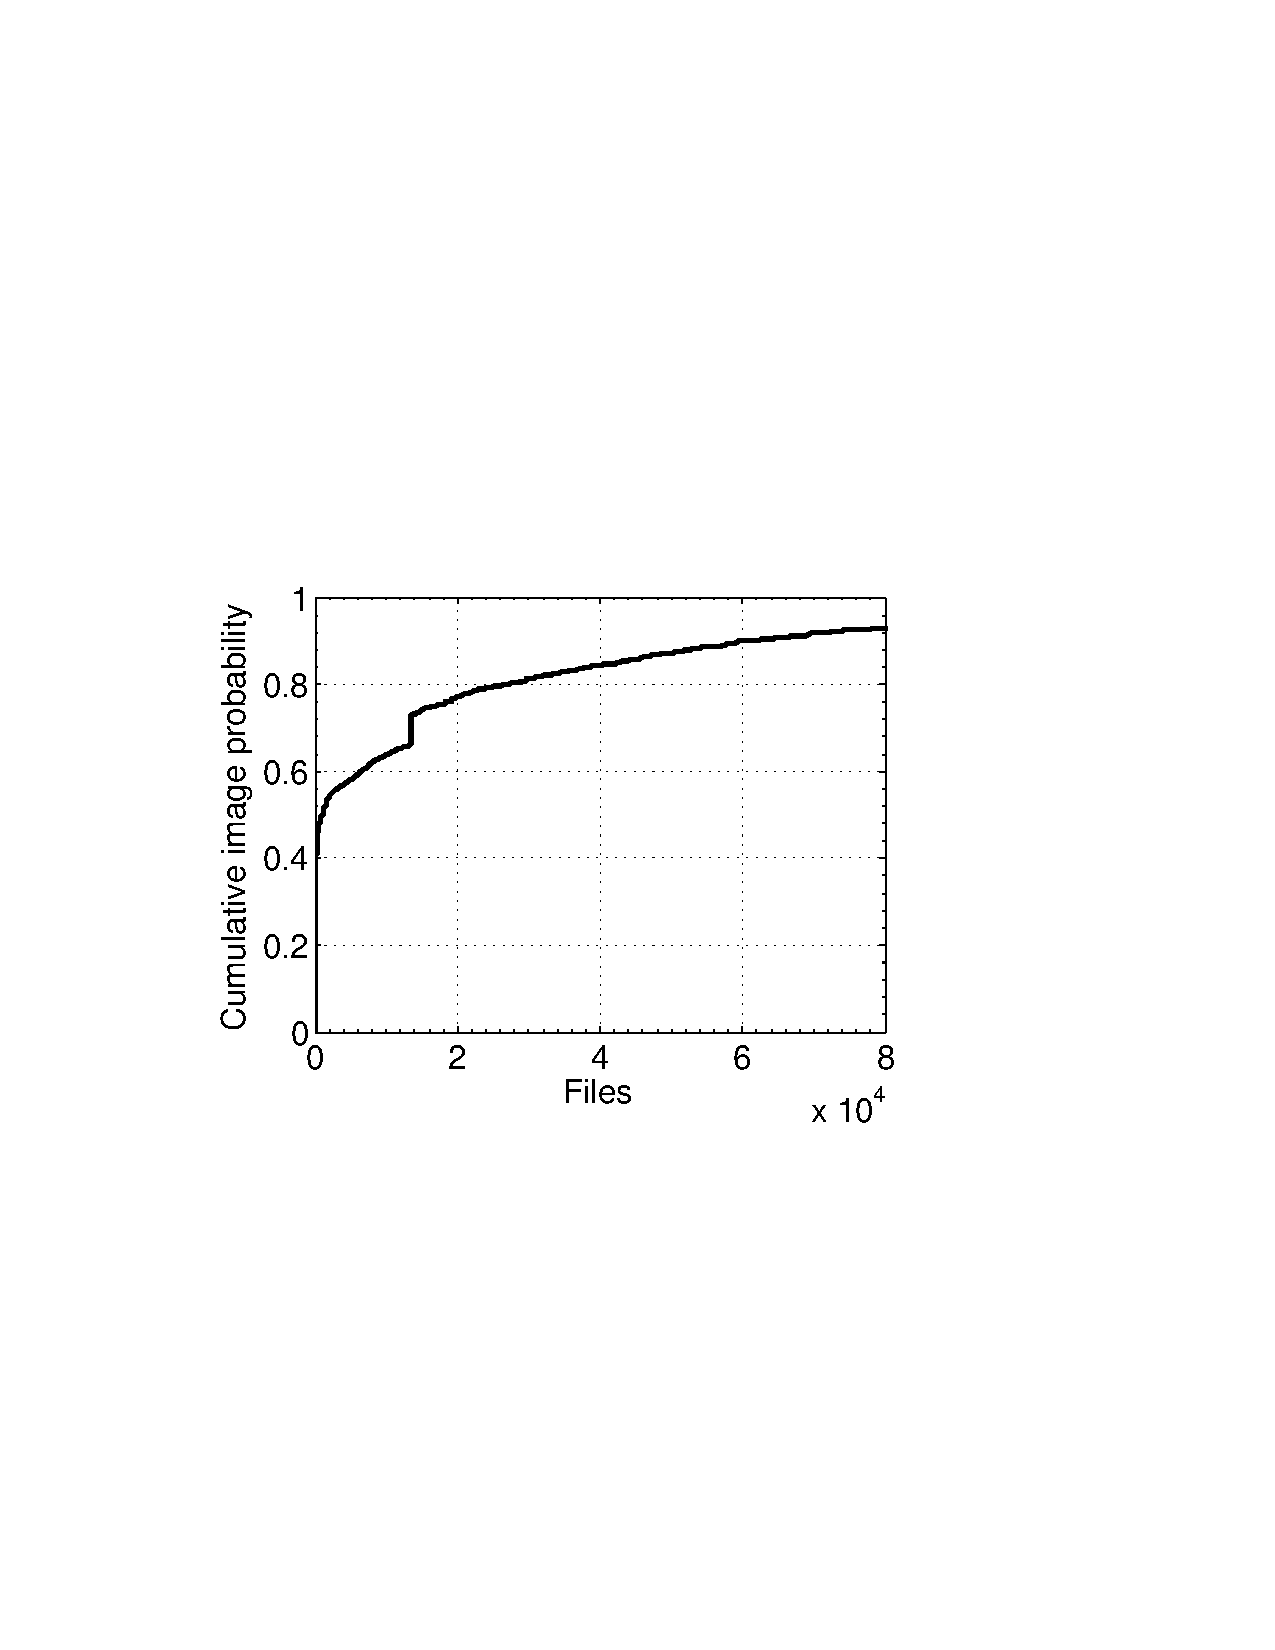
\includegraphics[width=1\textwidth]{graphs/file.pdf}
%		\caption{CDF of images by files}
%		\label{fig-file}
%	\end{minipage}
%\end{figure}

%\begin{figure}[htbp] 
%	\begin{minipage}{0.5\linewidth} 
%		\centering 
%		\includegraphics{circle} 
%		\caption{A Circle} 
%		\label{fig:circle} 
%	\end{minipage}% 
%	\begin{minipage}{0.5\linewidth} 
%		\centering 
%		\includegraphics{rectangle} 
%		\caption{A Rectangle} 
%		\label{fig:rectangle} 
%	\end{minipage} 
%\end{figure}
